\chapter{Diseño e implementación} % Main chapter title
\label{Chapter3} % Change X to a consecutive number; for referencing this chapter elsewhere, use \ref{ChapterX}
En este capítulo se detalla cómo se ha ejecutado la implementación del trabajo,
incluyendo la arquitectura del sistema, procesamiento de peticiones,
modelos extensos de lenguaje utilizados y las técnicas empleadas sobre la inteligencia artificial.
Adicionalmente, se incluyen los hallazgos intermedios significativos que fueron fundamentales para la implementación final.

\definecolor{mygreen}{rgb}{0,0.6,0}
\definecolor{mygray}{rgb}{0.5,0.5,0.5}
\definecolor{mymauve}{rgb}{0.58,0,0.82}

%%%%%%%%%%%%%%%%%%%%%%%%%%%%%%%%%%%%%%%%%%%%%%%%%%%%%%%%%%%%%%%%%%%%%%%%%%%%%
% parámetros para configurar el formato del código en los entornos lstlisting
%%%%%%%%%%%%%%%%%%%%%%%%%%%%%%%%%%%%%%%%%%%%%%%%%%%%%%%%%%%%%%%%%%%%%%%%%%%%%
\lstset{ %
  backgroundcolor=\color{white},   % choose the background color; you must add \usepackage{color} or \usepackage{xcolor}
  basicstyle=\footnotesize,        % the size of the fonts that are used for the code
  breakatwhitespace=false,         % sets if automatic breaks should only happen at whitespace
  breaklines=true,                 % sets automatic line breaking
  captionpos=b,                    % sets the caption-position to bottom
  commentstyle=\color{mygreen},    % comment style
  deletekeywords={...},            % if you want to delete keywords from the given language
  %escapeinside={\%*}{*)},          % if you want to add LaTeX within your code
  %extendedchars=true,              % lets you use non-ASCII characters; for 8-bits encodings only, does not work with UTF-8
  %frame=single,	                % adds a frame around the code
  keepspaces=true,                 % keeps spaces in text, useful for keeping indentation of code (possibly needs columns=flexible)
  keywordstyle=\color{blue},       % keyword style
  language=[ANSI]C,                % the language of the code
  %otherkeywords={*,...},           % if you want to add more keywords to the set
  numbers=left,                    % where to put the line-numbers; possible values are (none, left, right)
  numbersep=5pt,                   % how far the line-numbers are from the code
  numberstyle=\tiny\color{mygray}, % the style that is used for the line-numbers
  rulecolor=\color{black},         % if not set, the frame-color may be changed on line-breaks within not-black text (e.g. comments (green here))
  showspaces=false,                % show spaces everywhere adding particular underscores; it overrides 'showstringspaces'
  showstringspaces=false,          % underline spaces within strings only
  showtabs=false,                  % show tabs within strings adding particular underscores
  stepnumber=1,                    % the step between two line-numbers. If it's 1, each line will be numbered
  stringstyle=\color{mymauve},     % string literal style
  tabsize=2,	                   % sets default tabsize to 2 spaces
  title=\lstname,                  % show the filename of files included with \lstinputlisting; also try caption instead of title
  morecomment=[s]{/*}{*/}
}


%----------------------------------------------------------------------------------------
%	SECTION 1
%----------------------------------------------------------------------------------------
\section{Arquitectura del sistema}

Los primeros esfuerzos en el desarrollo del trabajo se enfocaron en definir el conjunto de módulos que compondrían la solución.
Estos componentes fueron identificados correctamente desde el principio:
un servidor \textit{web} y un módulo de modelos extensos de lenguaje.
Sin embargo, su relación en el sistema sí cambió durante la fase de implementación.

Inicialmente, durante la fase de diseño, se concibió que el servidor \textit{web} también alojaría el modelo extenso de lenguaje 
y sería responsable de gestionar su conjunto de datos, entrenamiento y despliegue.
Esta decisión se tomó al principio de la implementación,
influenciada por la forma en la que se trabaja con redes neuronales sencillas.
Hacer que esa arquitectura funcionase en este trabajo era mucho más complejo de lo estimado
por la propia naturaleza de los modelos extensos de lenguaje.
La incertidumbre generada por la ausencia de un conjunto de datos de calidad y tamaño suficientes,
y la dificultad implícita de reentrenar un modelo tan grande,
fueron un factor de riesgo permanente durante la fase de diseño.

Fue necesario profundizar en las materias de procesamiento de lenguaje natural y \textit{Large Language Models} \cite{fiubaLlm}
para definir una solución efectiva a este problema.
Finalmente se decidió por no solo ``extraer'' el módulo de modelos extensos de lenguaje del servidor \textit{web}
sino por simplificar su complejidad de programación haciendo uso de la herramienta LM Studio.
Este programa permite administrar los modelos locales de la computadora,
añadir nuevos a través de una interfaz de descarga
y hacer uso del hardware disponible para arrancarlos de forma transparente para el usuario.
Además, cuenta con varias ventanas de configuración de parámetros de lanzamiento del modelo, \textit{prompts} personalizados,
salida estructurada a través de un esquema JSON,
opciones relacionadas con la aleatoriedad y temperatura de la inferencia y otras características experimentales.

De este modo, el servidor \textit{web} también se simplificó en el desarrollo, ahorró mucho trabajo de programación sin
comprometer la calidad del proceso de la inteligencia artificial.
Esto también es coherente con la arquitectura de servidor ligero esperable en un prototipo
y tiene una mejor sinergia con bibliotecas orientadas al despliegue de servidores sencillos.

Tal y como se muestra en la figura \ref{fig:sist},
el prototipo es accesible para los clientes a través del protocolo HTTP-REST que expone el servidor.
Además, durante el desarrollo se implementó una sencilla página \text{web} para realizar peticiones de prueba
y mostrar la salida de texto obtenida.

\begin{figure}[htbp]
	\centering
	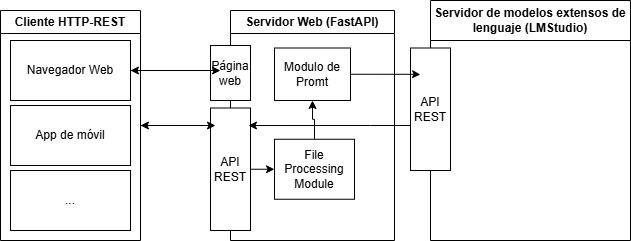
\includegraphics[width=0.9\textwidth]{./Figures/Sistema_es.png}
	\caption{Arquitectura del sistema.}
	\label{fig:sist}
\end{figure}

Otra ventaja de haber diseñado ambos módulos de forma independiente es que facilita al cliente
profundizar de forma paralela en los componentes sin comprometer el funcionamiento del resto del sistema.
Puede decidir si sustituir la implementación de uno u ambos módulos, escalarlos y distribuirlos en distintos entornos
para ajustarlo a su aplicación para \text{smartphones} y plan de expansión de servicios. 

%----------------------------------------------------------------------------------------
%	SECTION 2
%----------------------------------------------------------------------------------------
\section{Procesamiento de peticiones \textit{web} y ficheros}
Para la implementación del servidor web se decidió utilizar la biblioteca de FastAPI \cite{fastapi}.
Es una biblioteca moderna y de alto rendimiento para la construcción de APIs \text{web} en Python,
diseñada sobre estándares como OpenAPI \cite{openapi} y JSON schema.
Ofrece una forma rápida y eficiente de desarrollar interfaces REST
con una sintaxis sencilla y basada en anotaciones.
Esto permite una validación automática de datos de entrada y generación de documentación.
Todo esto hace que FastAPI sea una opción ideal para construir microservicios y prototipos rápidos.

El servidor expone dos servicios principales.
El primero es un \textit{endpoint} de tipo GET que proporciona la página \textit{web} que visualiza la interfaz gráfica del prototipo.
El otro servicio implementa un método POST para recibir las peticiones de consulta por parte del usuario para su procesamiento
y reenvío al módulo de inteligencia artificial. 


\pagebreak
\subsection{Procesamiento de peticiones}
En la figura \ref{fig:flux} se representa el diagrama de flujo correspondiente al manejo de las peticiones entrantes.

\begin{figure}[htbp]
	\centering
	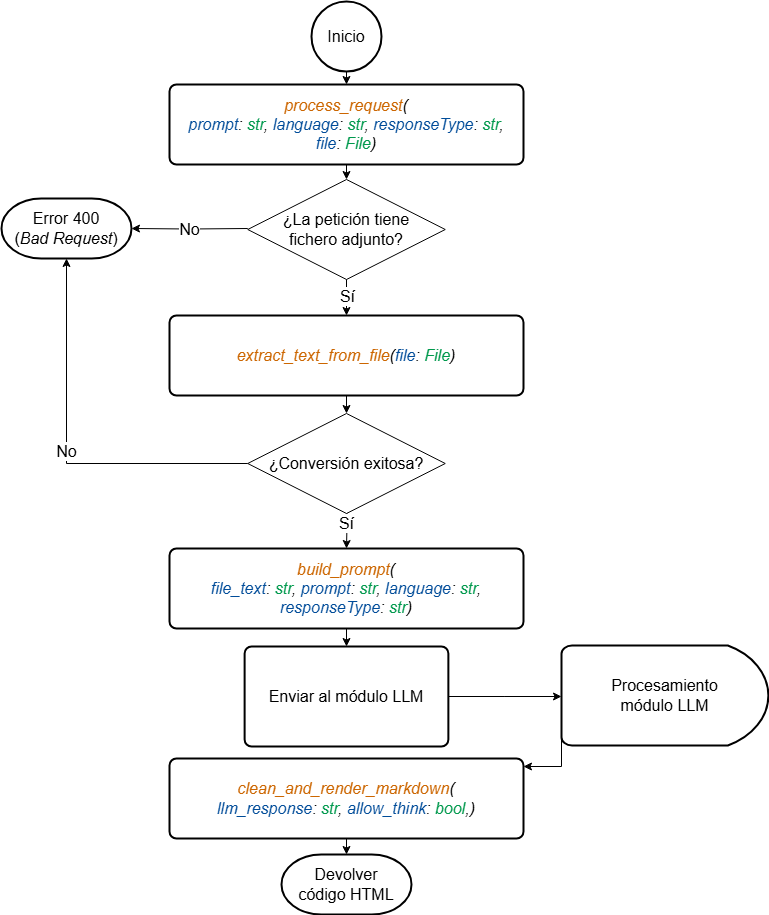
\includegraphics[width=1\textwidth]{./Figures/flux-diagram.png}
	\caption{Diagrama de flujo del procesamiento de peticiones.}
	\label{fig:flux}
\end{figure}

El proceso comienza cuando el cliente envía una solicitud con los datos de consulta a través de un cliente REST.
Esto puede ser a través del formulario proporcionado por el servidor o a través de cualquier otra herramienta como,
por ejemplo, PostMan.
Tras realizar las comprobaciones iniciales,
el servidor continúa procesando la información mediante una serie de funciones específicas:
\begin{itemize}
\item \texttt{extract\_text\_from\_file}:
es el proceso encargado de extraer la información textual de los ficheros adjunto
y formatearlo para que el módulo de modelos extensos de lenguaje sea capaz de interpretarlo.
En esta función se hace uso de las bibliotecas de cgardet, docx y fitz para la detección del formato y
su conversión a texto plano.
\item \texttt{build\_prompt}:
esta función es la encargada de construir el \textit{prompt} a partir del texto extraído del fichero
y las entradas adicionales proporcionadas por el usuario, entre las que se incluyen el idioma de
la respuesta, el tipo de listado que se solicita y algunas instrucciones adicionales.
En esta función se emplea la ingeniería de \textit{prompting} que se envía posteriormente al módulo LLM.
Se detalla más adelante en la sección (FALTA AÑADIR REFERENCIA)
\item \texttt{clean\_and\_render\_markdown}:
esta función se encarga de limpiar la salida y formatearla en código HTML
a través de la biblioteca markdown para una mejor legibilidad en navegadores web.
\end{itemize}

Cabe destacar que para la comunicación con el módulo LLM,
aunque LM Studio ofrece un SDK en Python para interactuar mediante programación,
se optó por utilizar su interfaz REST.
La razón es que así el servidor \textit{web} no depende exclusivamente de la biblioteca de LM Studio.
Al emplear un protocolo de comunicación estándar como REST,
el servidor web puede interactuar fácilmente con cualquier otro servicio que aloje modelos extensos de lenguaje,
lo que le da mayor flexibilidad.

\subsection{Interfaz gráfica}
El servidor también facilita el acceso a una página \textit{web} con la interfaz gráfica del prototipo,
tal y como se aprecia en la figura \ref{fig:webPage}.

\begin{figure}[htbp]
	\centering
	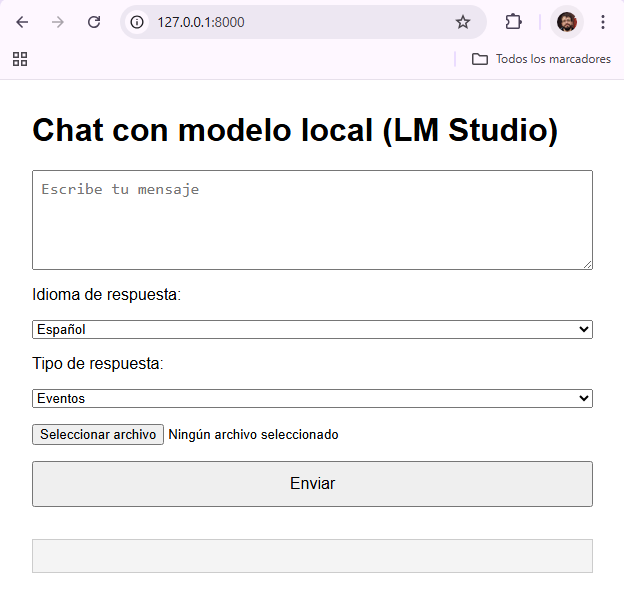
\includegraphics[width=0.8\textwidth]{./Figures/webpage.png}
	\caption{Interfaz gráfica del prototipo.}
	\label{fig:webPage}
\end{figure}

El formulario consta de los siguientes elementos:
\begin{itemize}
\item Cuadro de texto:
este elemento se utiliza para darle las instrucciones específicas a la inteligencia artificial.
Está pensado para que sea un mensaje breve y conciso que pueda ayudar al usuario a guiar un poco mejor la respuesta.
Es un parámetro opcional y puede dejarse en blanco.
\item Idioma de respuesta:
se trata de un \textit{combobox} que contiene dos opciones: inglés y español.
El módulo LLM responderá en el idioma seleccionado, independientemente del idioma del fichero de entrada.
Este elemento se añadió porque algunos modelos presentan comportamientos anómalos si responden en un idioma distinto al inglés.
\item Tipo de respuesta:
permite a la inteligencia artificial centrar su respuesta en un aspecto concreto de la narrativa.
Al estar instruida en devolver listas de elementos, la idea es que el usuario pueda elegir la opción
específica de la creación de mundos que le interese.
\item Fichero adjunto:
es el elemento más importante del formulario.
El usuario puede agregar un fichero con el contexto narrativo existente
y enviarlo a la inteligencia artificial para que genere nuevo contenido.
\end{itemize}
% En las siguientes secciones se detallan las funciones de cada módulo y el trabajo realizado.

% Se puede agregar código o pseudocódigo dentro de un entorno lstlisting con el siguiente código:

% \begin{verbatim}
% \begin{lstlisting}[caption= "un epígrafe descriptivo"]
% 	las líneas de código irían aquí...
% \end{lstlisting}
% \end{verbatim}

% A modo de ejemplo:

% \begin{lstlisting}[label=cod:vControl,caption=Pseudocódigo del lazo principal de control.]  % Start your code-block

% #define MAX_SENSOR_NUMBER 3
% #define MAX_ALARM_NUMBER  6
% #define MAX_ACTUATOR_NUMBER 6

% uint32_t sensorValue[MAX_SENSOR_NUMBER];		
% FunctionalState alarmControl[MAX_ALARM_NUMBER];	//ENABLE or DISABLE
% state_t alarmState[MAX_ALARM_NUMBER];						//ON or OFF
% state_t actuatorState[MAX_ACTUATOR_NUMBER];			//ON or OFF

% void vControl() {

% 	initGlobalVariables();
	
% 	period = 500 ms;
		
% 	while(1) {

% 		ticks = xTaskGetTickCount();
		
% 		updateSensors();
		
% 		updateAlarms();
		
% 		controlActuators();
		
% 		vTaskDelayUntil(&ticks, period);
% 	}
% }
% \end{lstlisting}



